\section{Systemmodelle}

\subsection{Szenarien}

\subsubsection{Eigenes Spiel erstellen}
Der Benutzer möchte ein Spiel erstellen, das beide Spieler dafür belohnt, unterschiedliche Entscheidungen zu treffen.\\
Hierfür öffnet er das Spiele-Menü und klickt auf 'neues Spiel'. Er gibt dem Spiel einen Namen und setzt die Werte:
\begin{table}[H]
\centering
\setlength{\extrarowheight}{2pt}
\begin{tabular}{cc|c|c|}
  & \multicolumn{1}{c}{} & \multicolumn{2}{c}{Spieler $2$} \\
  & \multicolumn{1}{c}{} & \multicolumn{1}{c}{$K$} & \multicolumn{1}{c}{$D$} \\\cline{3-4}
  \multirow{2}*{Spieler $1$} & $K$ & $0,0$ & $3,3$ \\\cline{3-4} 
  & $D$ & $3,3$ & $0,0$ \\\cline{3-4}
\end{tabular}
\end{table}
Anschließend versieht er sein Spiel mit einer Beschreibung.\\
Er beendet den Vorgang durch Klicken von 'Änderungen speichern und schließen'.

\subsubsection{Kombinierte Strategie erstellen}
Der Benutzer möchte eine eigene kombinierte Strategie erstellen, bei der Agenten eine besondere Verhaltensweise gegenüber Agenten innerhalb ihrer Gruppe und gegenüber reicheren Agenten außerhalb ihrer Gruppe haben.\\
Hierfür öffnet er das Spiele-Menü und klickt auf 'neue kombinierte Strategie'. Er gibt der Strategie den Namen "`GruppenTitforTat"'. Unter 'Bedingungen' klickt er auf 'hinzufügen'. Er wählt die Bedingung 'Mit meiner Gruppe' und die Strategie 'Tit for Tat'.
Analog fügt er eine weitere Bedingung 'Mit reicheren Agenten' mit der Strategie 'Grim' hinzu. Für 'keine Bedingung' wählt er 'keine Kooperation'. Schließlich beschreibt er in einem Textfeld seine Strategie und klickt 'kombinierte Strategie speichern und schließen'.

\subsubsection{Rivalisierende Gruppen}
Der Benutzer möchte eine Population mit zwei rivalisierenden Gruppen simulieren.\\
Hierfür hat er bereits eine kombinierte Strategie erstellt, nach der Agenten mit Agenten aus ihrer eigenen Gruppe kooperieren, mit Agenten aus einer anderen Gruppe nicht kooperieren und sonst 'Tit for Tat' spielen.\\
Im Initialisierungsmenü erstellt er nun zwei Gruppen und gibt unter 'Anteil aller Agenten' den Wert 25 ein. Beiden Gruppen weist er seine Strategie zu, allen anderen 'Tit for Tat'.

\subsubsection{Ausreißer im Ergebnis vermeiden}
Der Benutzer hat sich für eine bestimmte Konfiguration entschieden, mit der er eine Simulation durchführen möchte. Um das Risiko von Ausreißern im Ergebnis zu verringern, wählt er beim Start der Simulation eine hohe Wiederholungsanzahl aus. Nach die Simulation abgeschlossen ist, wählt er in der Ergebnisansicht unter 'Wiederholung' den Punkt 'Durchschnitt' aus.

\newpage

\subsection{Anwendungsfälle}

\begin{figure}[htbp]
{\centering 
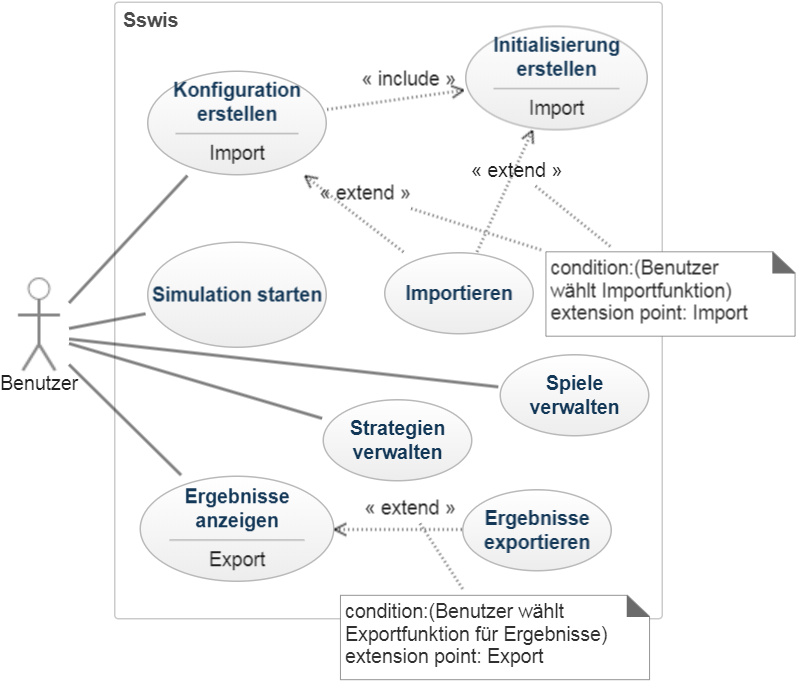
\includegraphics[width=0.8\textwidth]{Anwendungsfalldiagramme/usecase_sswis2.png}
\caption{Die grundlegenden Anwendungen des Programms} }
\bigskip
Sswis ist ein Simulator und gliedert sich als solcher in drei übergeordnete Anwendungen. Die Konfiguration der Rahmenbedingungen, das Starten der eigentlichen Simulation und das Abrufen der Ergebnisse. Die Interaktion mit dem Benutzer beschränkt sich im Wesentlichen auf die Konfiguration und die Anzeige der Ergebnisse. Außerdem kann er die für die Konfiguration verfügbaren Spiele und Strategien verwalten\footnotemark. Die Simulation wird vom Benutzer initiiert und läuft anschließend ohne weiteres Einwirken von außen ab.

Auf der technischen Seite ist das Importieren von Konfigurationen und Initialisierungen sowie das Exportieren von Ergebnissen in Form jeweils einer Textdatei (z.B. CSV; Comma-separated values) möglich. Dateien zum Import einer Konfiguration bzw. Initialisierung wurden zu einem früheren Zeitpunkt durch den entsprechenden Assistenten erstellt.

\end{figure}

\footnotetext{darin inbegriffen sind Möglichkeiten zur Erstellung, Benennung und Löschung sowohl von Spielen als auch von Strategien}